\documentclass[12pt, oneside]{book}

% Paquetes necesarios
\usepackage{graphicx}
\usepackage{titlesec}
\usepackage{subcaption}
\usepackage{hyperref}
\usepackage{natbib}

\usepackage{float}

% Configuración de la página
\usepackage[a4paper, top=2.5cm, bottom=2.5cm, left=3cm, right=2.5cm]{geometry}

% Configuración de la carpeta de imágenes
\graphicspath{{images/}}

% Configuración del formato de los capítulos
\titleformat{\chapter}[display]
{\normalfont\huge\bfseries}{\chaptertitlename\ \thechapter}{20pt}{\Huge}

% Información de la tesis
\newcommand{\university}{Universidad Complutense de Madrid}
\newcommand{\facultad}{Facultad de Estudios Estadísticos}
\newcommand{\master}{Máster Big Data y Data Science}
\newcommand{\thesisTitle}{Detección y segmentación de tumores cerebrales en imágenes de resonancia magnética con técnicas de Deep Learning}
\newcommand{\authorName}{MSc. Carlos Gordillo Olivera}
\newcommand{\thesisYear}{2024}



% Cambiar nombres en español
\renewcommand{\chaptername}{Capítulo}
\renewcommand{\contentsname}{Índice}

\begin{document}

% Portada
\begin{titlepage}
    \centering
    %\vspace*{2cm}
    
    {\LARGE\textbf{\university}\par}
    %\vspace{0.5cm}
        {\Large\textbf{\facultad}\par}
         {\Large\textbf{\master}\par}
    \vspace{1cm}
    
        
\includegraphics[width=4.5cm]{images/UCM-Logo.png}
    \vspace*{1cm}
    
    {\huge\textbf{\thesisTitle}\par}
    \vspace{7cm}
    
    {\Large\textbf{\authorName}\par}
    \vfill
    
    {\Large\textbf{\thesisYear}\par}
    
\end{titlepage}

% Índice
\tableofcontents

% Capítulos
%\chapter{Introducción}
% Introducción

\chapter{Introducción}


\section{Imágenes por resonancia magnética}

La utilización de imágenes por resonancia magnética (MRI) ha revolucionado el campo de la neurología al proporcionar una visión detallada y no invasiva del cerebro y sus estructuras. La capacidad de obtener imágenes de alta resolución de los tejidos cerebrales en diferentes planos anatómicos ha permitido a los médicos y investigadores diagnosticar y tratar una amplia gama de trastornos neurológicos con mayor precisión y efectividad. 

La MRI es especialmente invaluable en el estudio de enfermedades cerebrales como los tumores, los accidentes cerebrovasculares, las enfermedades neurodegenerativas y los trastornos del desarrollo cerebral. Estas imágenes proporcionan información crucial sobre la localización, el tamaño, la extensión y la naturaleza de las anomalías cerebrales, lo que ayuda a los médicos a planificar intervenciones quirúrgicas, a diseñar estrategias de tratamiento y a realizar un seguimiento preciso de la progresión de la enfermedad.

Además, la MRI ofrece la capacidad única de detectar cambios sutiles en la estructura y la función del cerebro que pueden no ser visibles en otros tipos de imágenes médicas. Esto es fundamental para comprender la fisiopatología de las enfermedades cerebrales, identificar biomarcadores tempranos de enfermedades y evaluar la eficacia de los tratamientos.

Para una profundización mayor de los conceptos físicos detrás de esta técnica de imágenes recurrir a la \href{https://ricabib.cab.cnea.gov.ar/774/}{tesis de maestría}.

\section{Tumores cerebrales: generalidades}

Se dice que un tumor cerebral es una masa de células que se forma en el tejido cerebral o en ubicaciones cercanas a este, incluyendo los nervios, glándula pituitaria, glándula pineal y las meninges, como se muestra en la Fig. \ref{fig.cerebros}.

\begin{figure}[H]
    \centering
    \begin{subfigure}[b]{0.45\linewidth}
        \centering
        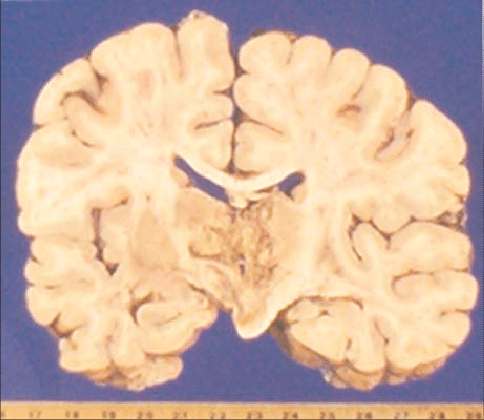
\includegraphics[width=0.75\linewidth]{chapters/introduccion/images/normal.jpg}
        \caption{Cerebro sano}
    \end{subfigure}
    \hspace{0.5cm}
    \begin{subfigure}[b]{0.45\linewidth}
        \centering
        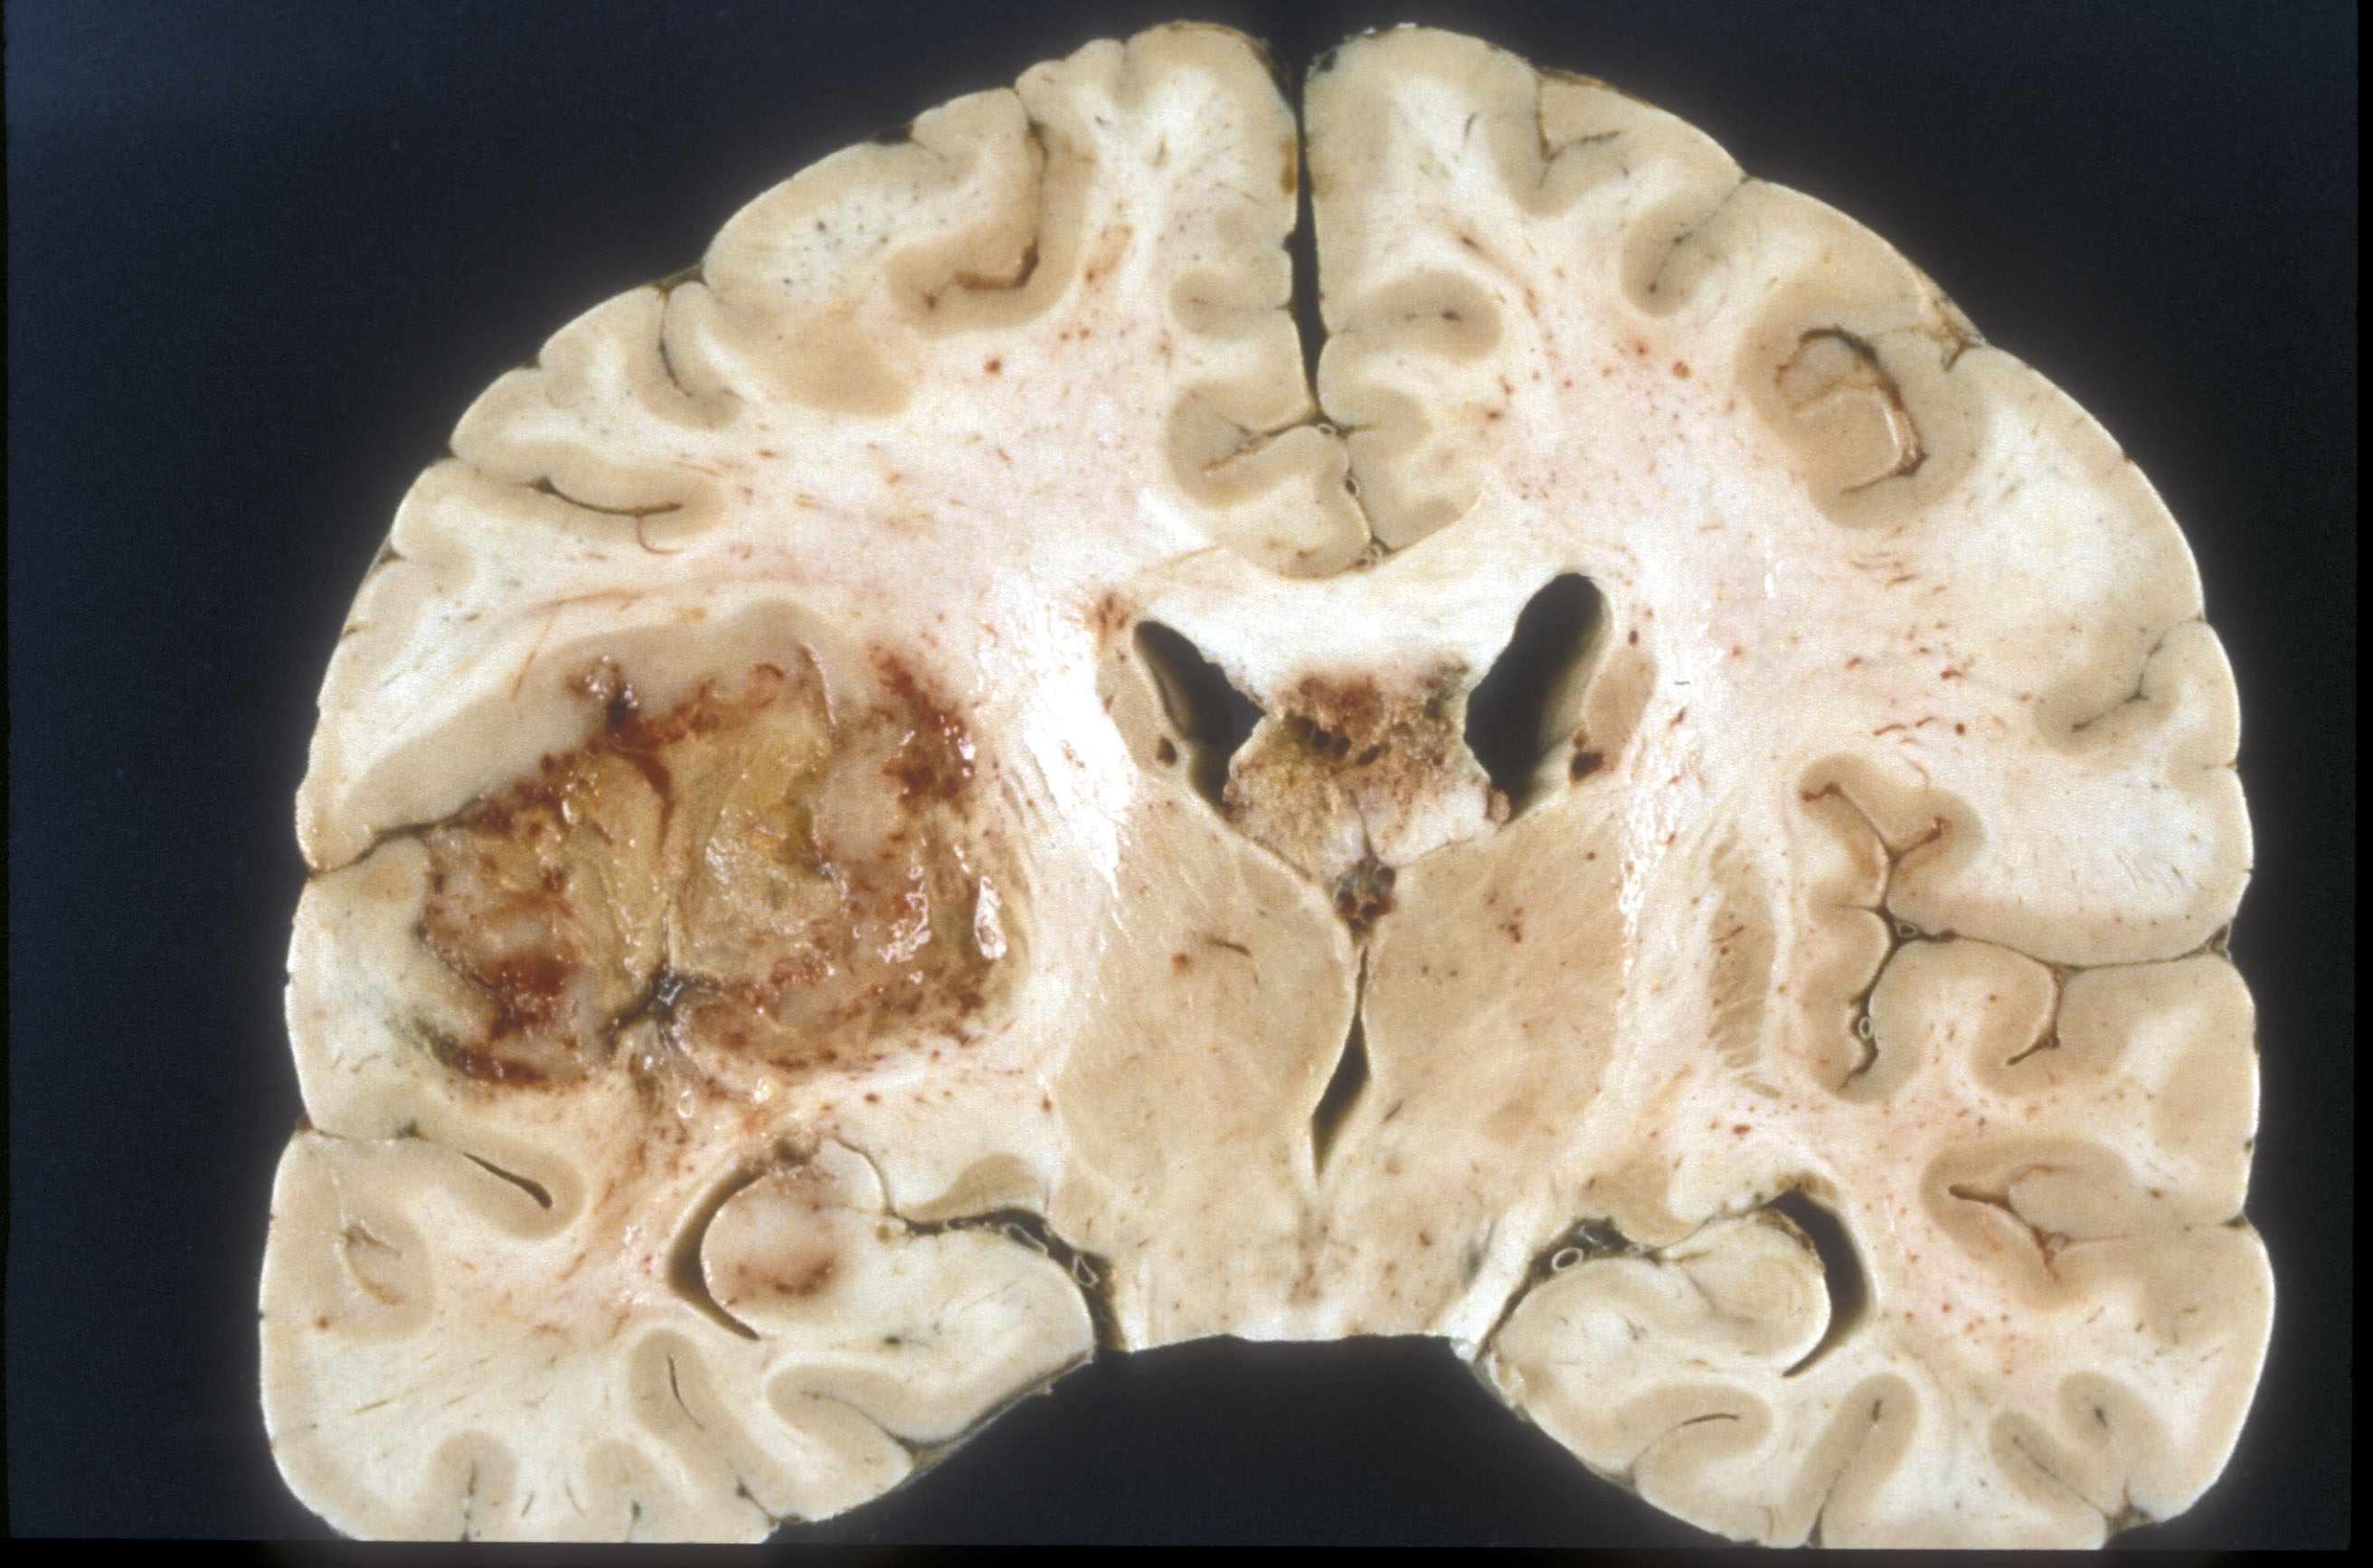
\includegraphics[width=\linewidth]{chapters/introduccion/images/tumor.jpg}
        \caption{Cerebro con tumor}
    \end{subfigure}
    \caption{Corte coronal de cerebro ex vivo sano y con un tumor.}
    \label{fig.cerebros}
\end{figure}

Los tumores cerebrales se pueden clasificar en primarios o secundarios, dependiendo de si se originan en el propio cerebro o se diseminan desde otra parte del cuerpo (también conocidos como metastásicos). Estas estructuras pueden variar en tamaño, donde algunos, incluso pequeños, pueden provocar síntomas graves y evidentes, mientras que otros de mayor tamaño pueden pasar desapercibidos debido a la falta de síntomas.

En términos generales, algunos tumores primarios son benignos, lo que significa que no son cancerosos. Sin embargo, con el tiempo, pueden crecer y afectar el tejido cerebral circundante al comprimirlo. Por el contrario, los tumores cancerosos pueden desarrollarse de manera rápida y agresiva, invadiendo y destruyendo el tejido cerebral sano a su alrededor.

\section{Motivación del trabajo}

La detección y segmentación de tumores cerebrales representan una tarea de gran importancia en el ámbito médico, según lo indicado por la Organización Mundial de la Salud (OMS). La capacidad de identificar y delimitar con precisión la ubicación y extensión de estos tumores es fundamental para la planificación de intervenciones quirúrgicas efectivas. La resección quirúrgica de los tumores cerebrales depende en gran medida de una detección temprana y una segmentación precisa, lo que puede significar la diferencia entre la vida y la muerte, así como entre la salud y la discapacidad permanente para los pacientes. Además, la detección oportuna de estos tumores permite iniciar el tratamiento adecuado en las etapas iniciales de la enfermedad, lo que puede mejorar significativamente los resultados clínicos y la calidad de vida de los pacientes al evitar complicaciones graves y preservar las funciones cerebrales vitales.

En este contexto, las técnicas de inteligencia artificial y aprendizaje profundo han emergido como herramientas poderosas y prometedoras. La aplicación de algoritmos de inteligencia artificial, como las redes neuronales convolucionales, permite procesar grandes volúmenes de datos de imágenes médicas de manera rápida y precisa, facilitando la identificación automática de características relevantes y la segmentación precisa de los tejidos tumorales. El uso de estas herramientas no solo agiliza el proceso de diagnóstico, sino que también mejora la precisión y fiabilidad de las predicciones, lo que puede conducir a una detección más temprana y un tratamiento más efectivo de los tumores cerebrales. En última instancia, la integración de la inteligencia artificial y las técnicas de aprendizaje profundo en la práctica clínica tiene el potencial de revolucionar el manejo de esta enfermedad, mejorando los resultados clínicos y la calidad de vida de los pacientes.

\section{Organización del Documento}

La organización del documento se estructura en dos partes principales. En la primera parte, se aborda la detección de tumores cerebrales, mientras que la segunda parte se centra en la segmentación de los mismos. Cada una de estas partes se desarrolla en un capítulo independiente, donde se discuten los fundamentos teóricos, las metodologías utilizadas y los resultados obtenidos en cada etapa del proceso.

Tras la presentación de los resultados, se procede a realizar un análisis detallado de las métricas correspondientes, evaluando la efectividad y precisión de los modelos desarrollados en la detección y segmentación de los tumores cerebrales. Este análisis se realiza con el objetivo de validar el rendimiento de los algoritmos y determinar su utilidad en la práctica clínica.

Finalmente, en el último capítulo del documento, se describe el diseño e implementación de una API y una página web interactiva sencilla. Estas herramientas permiten a los usuarios interactuar con los modelos desarrollados, facilitando su uso en entornos clínicos y de investigación. Se detallan las funcionalidades y características de la API y la página web, así como los pasos necesarios para su implementación y utilización efectiva.

Todos los detalles de código, armado de modelos, cálculo de métricas, procesamiento de datos, así como la implementación de la API y front end se encuentra en el \href{https://github.com/carlosng95/UCM-TFM}{Github}.









% Introducción

\chapter{Detección de tumores}

Link del dataset: https://www.kaggle.com/datasets/preetviradiya/brian-tumor-dataset/data

\section{Descripción del dataset}

La metadata informa que el dataset contiene 4600 imágenes en total, divididas en dos clases: $tumor$ y $normal$ según se observa en la Fig. \ref{fig.clases}. En este contexto va a entenderse a $normal$ como $sin$ $tumor$, pero no significa que no existan otras patologías por ejemplo isquemias.

\begin{figure}[H]
\centering
        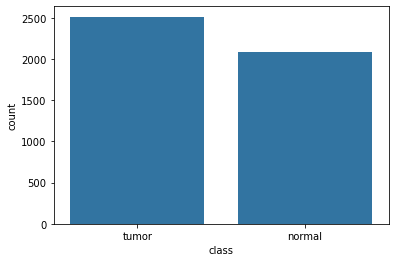
\includegraphics[width=0.5\linewidth]{chapters/deteccion/images/clases.png}
        \caption{Distribución de clases de imágenes del dataset para detección.}
        \label{fig.clases}
  \end{figure}


En la Fig. \ref{fig:conjunto_imagenes} se observan algunas imágenes del dataset. En particular, las Fig. \ref{fig:normal1}, \ref{fig:normal2} y \ref{fig:normal3} corresponden a pacientes normales mientras que las Fig. \ref{fig:tumor1}, \ref{fig:tumor2} y \ref{fig:tumor3} corresponden a pacientes con tumor cerebral. 

\begin{figure}[H]
    \centering
    \begin{subfigure}[b]{0.3\textwidth}
        \centering
        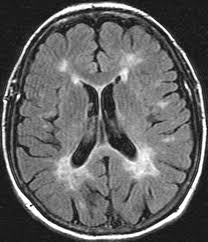
\includegraphics[width=\linewidth]{chapters/deteccion/images/sano1.jpg}
        \caption{Axial T2 flair con isquemias periventriculares. Normal.}
        \label{fig:normal1}
    \end{subfigure}
    \hfill
    \begin{subfigure}[b]{0.3\textwidth}
        \centering
        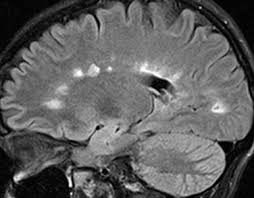
\includegraphics[width=\linewidth]{chapters/deteccion/images/sano2.jpg}
        \caption{Sagital T2 flair. Isquemias.}
        \label{fig:normal2}
    \end{subfigure}
    \hfill
    \begin{subfigure}[b]{0.3\textwidth}
        \centering
        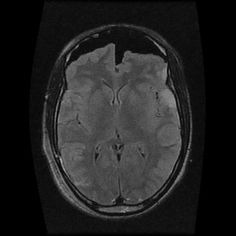
\includegraphics[width=\linewidth]{chapters/deteccion/images/sano3.jpg}
        \caption{Axial T2 flair. Normal.}
        \label{fig:normal3}
    \end{subfigure}
    
    \vspace{0.5cm}
    
    \begin{subfigure}[b]{0.3\textwidth}
        \centering
        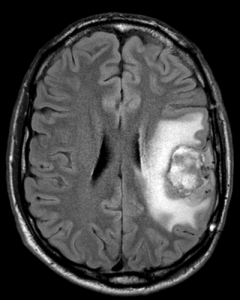
\includegraphics[width=\linewidth]{chapters/deteccion/images/cancer1.png}
        \caption{Axial T2 flair. Tumor.}
        \label{fig:tumor1}
    \end{subfigure}
    \hfill
    \begin{subfigure}[b]{0.3\textwidth}
        \centering
        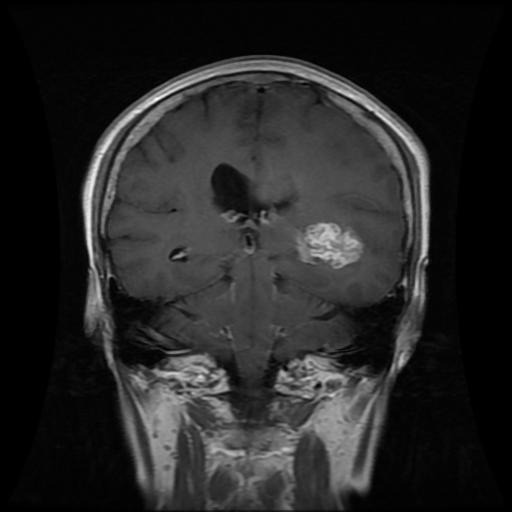
\includegraphics[width=\linewidth]{chapters/deteccion/images/cancer2.jpg}
        \caption{Coronal T1 con contraste. Tumor.}
        \label{fig:tumor2}
    \end{subfigure}
    \hfill
    \begin{subfigure}[b]{0.3\textwidth}
        \centering
        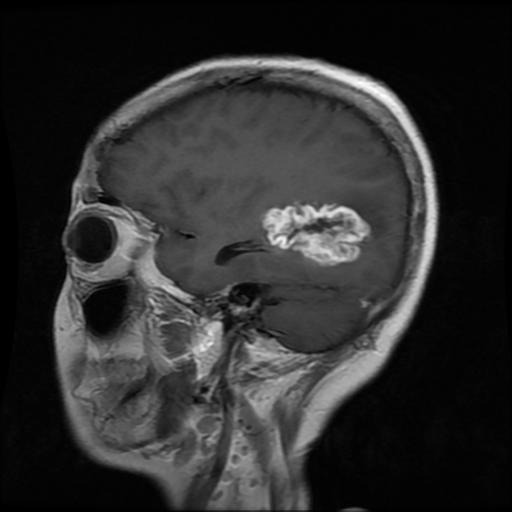
\includegraphics[width=\linewidth]{chapters/deteccion/images/cancer3.jpg}
        \caption{Sagital T1 con contraste. Tumor.}
        \label{fig:tumor3}
    \end{subfigure}
    \caption{Muestra de imágenes del dataset.}
    \label{fig:conjunto_imagenes}
\end{figure}

Es interesante notar que la Fig. \ref{fig:normal1} es un corte axial $T_2$ flair de cerebro donde claramente se observa una anormalidad del tejido. Las zonas hiperintensas (blancas) que rodean a los ventrículos de forma bilateral corresponden a isquemias típicas de la edad pero no es un tumor, por lo tanto la imagen es clasificada como de paciente sano. 

Por otro lado, una patología isquémica también se observa en la Fig. \ref{fig:tumor1}, en este caso está rodeando a un tumor. Por lo tanto, esta imagen se clasifica como tumoral. 

\section{Preprocesamiento de las imágenes}

Las imágenes disponibles tenían no solo diferentes tamaños sino también diferentes relaciones de aspecto. La Fig. \ref{fig.relaciones} muestra la distribución de tamaños, la recta roja corresponde a imágenes que sean cuadradas.

\begin{figure}[H]
\centering
        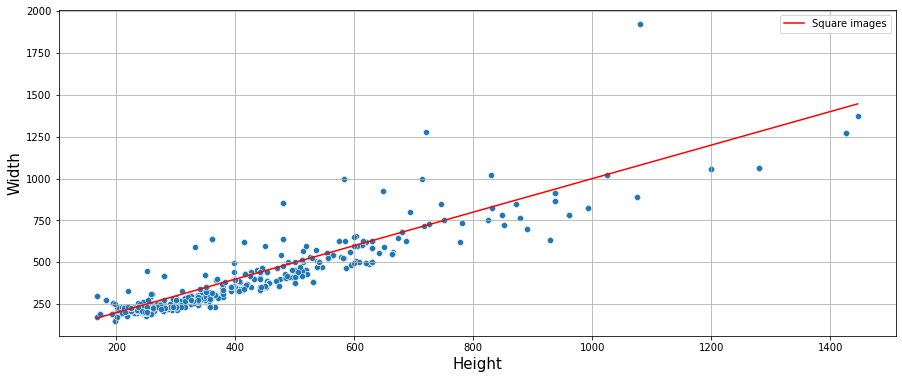
\includegraphics[width=\linewidth]{chapters/deteccion/images/relaciones.png}
        \caption{Tamaños de las imágenes del dataset}
        \label{fig.relaciones}
  \end{figure}

Con el objetivo de normalizar las imágenes, se optó por redimensionarlas a una resolución de $256 \times 256$ píxeles. 

Además, se aplicó una conversión a escala de grises, dado que esta representación es ampliamente utilizada en el ámbito del diagnóstico médico, garantizando así una compatibilidad estándar para el análisis y la interpretación de las imágenes.

Un último preprocesamiento que se aplicó es normalizar el rango de valores de los píxeles de la imagen, originalmente cada píxel $p_{ij}\in [0,255]$ y luego de la transformación $p_{ij}\in [0,1]$.

\section{Modelos}

Antes de aplicar los diferentes modelos se realizó la partición en $train/test$ en una proporción $80/20$. 

Las variables predictoras son los propios píxeles de cada imagen, mientras que el target es binario: tumor/sano. 

Inicialmente se aplicaron modelos tradicionales de $\textit{machine learning}$. Para estos modelos anteriores se realizó un preprocesamiento más, la conversión de las imágenes en formato de matriz ($256\times256$) a vector de dimensión $256\cdot256=65536$. Los modelos trabajados fueron:

\begin{itemize}
\item Naive bayes
\item Random Forest Classifier
\item Logistic Regression
\item Decision Tree Classifier
\item KNN
\end{itemize}.


\subsection{Naive bayes}

Este modelo por ser el más simple de todos constituye un baseline. Luego del entrenamiento se obtuvieron la matriz de confusión y curva roc tanto para train como para test, las cuales son mostradas en la Fig. \ref{fig.naive}. 

\begin{figure}[H]
\centering
        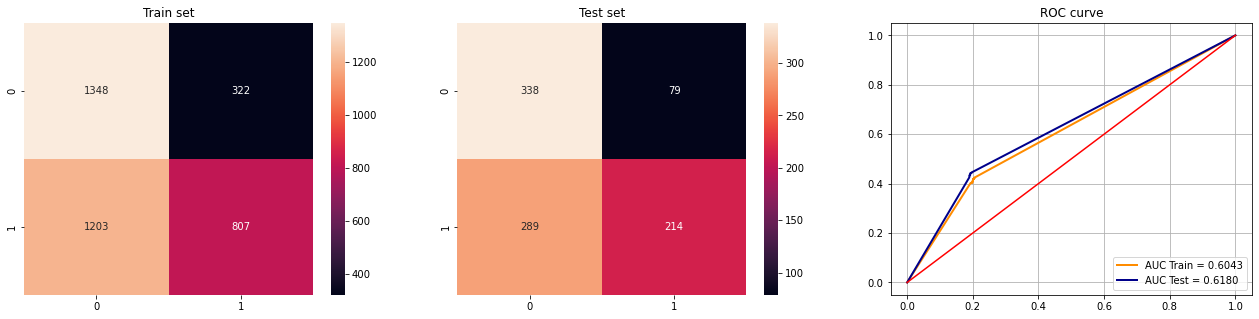
\includegraphics[width=\linewidth]{chapters/deteccion/images/naive.png}
        \caption{Métricas para el modelo Naive-Bayes}
        \label{fig.naive}
  \end{figure}
  
  En la Tabla \ref{tabla.naive} se detallan las métricas derivadas de la matriz de confusión. Se observa que las métricas son bajas, lo cual es coherente con que es un modelo demasiado simple. 

\begin{table}[H]
\centering
\begin{tabular}{|c|c|c|c|c|c|}
\hline
      & Accuracy & Precision & Recall & AUC    & $F_1$ score \\ \hline
Train & 0.5856   & 0.7148    & 0.4015 & 0.6043 & 0.5142      \\ \hline
Test  & 0.6      & 0.7304    & 0.4254 & 0.618  & 0.5377      \\ \hline
\end{tabular}
\caption{Métricas para el modelo Naive-Bayes}
\label{tabla.naive}
\end{table}

\subsection{Random forest}

Luego del entrenamiento se obtuvieron la matriz de confusión y curva roc tanto para train como para test, las cuales son mostradas en la Fig. \ref{fig.rf}. 

\begin{figure}[H]
\centering
        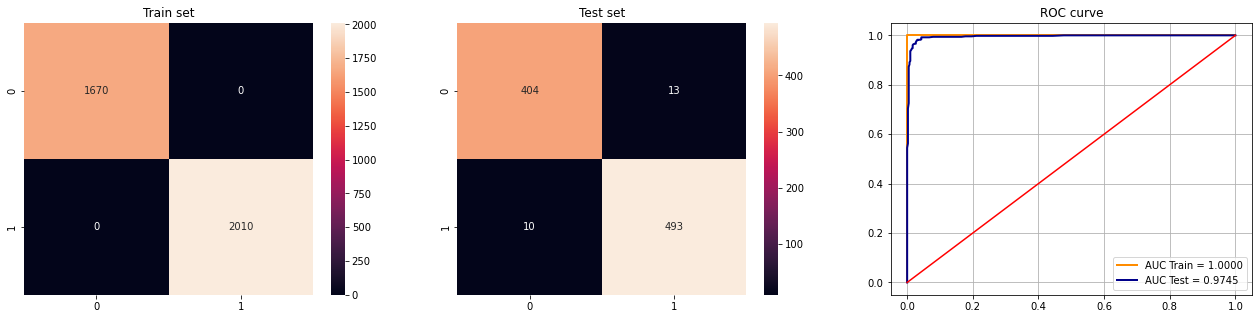
\includegraphics[width=\linewidth]{chapters/deteccion/images/rf.png}
        \caption{Métricas para el modelo Random Forest}
        \label{fig.rf}
  \end{figure}
  
 En la Tabla \ref{tabla.rf} se detallan las métricas derivadas de la matriz de confusión. Se observa que las métricas son bajas, lo cual es coherente con que es un modelo demasiado simple. 

\begin{table}[H]
\centering
\begin{tabular}{|c|c|c|c|c|c|}
\hline
      & Accuracy & Precision & Recall & AUC    & $F_1$ score \\ \hline
Train & 1.0   & 1.0    & 1.0 & 1.0 & 1.0      \\ \hline
Test  & 0.975      & 0.9743    & 0.9801 & 0.9745  & 0.9772      \\ \hline
\end{tabular}
\caption{Métricas para el modelo Random Forest}
\label{tabla.rf}
\end{table}

Es notable que este modelo resulta perfecto para el conjunto de entrenamiento, lo cual haría sospechar de un posible overfitting, pero viendo las métricas correspondientes al conjunto de test esto parecería estar descartado. 


\subsection{Logistic regression}

Luego del entrenamiento se obtuvieron la matriz de confusión y curva roc tanto para train como para test, las cuales son mostradas en la Fig. \ref{fig.lr}. 

\begin{figure}[H]
\centering
        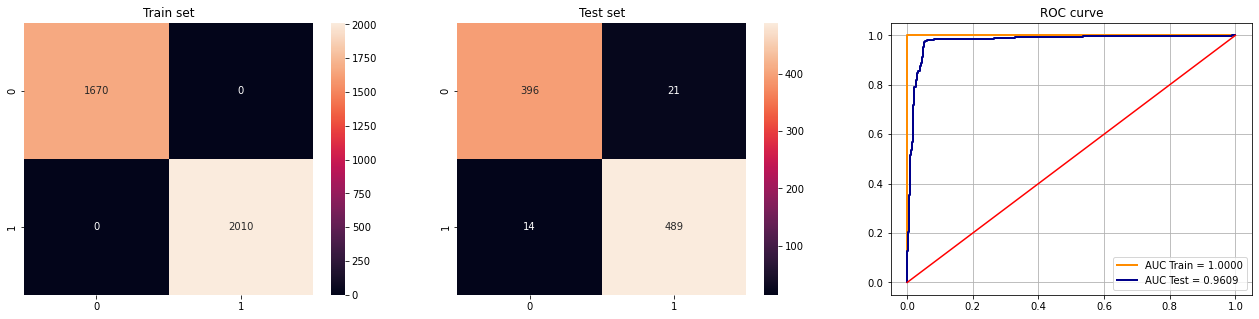
\includegraphics[width=\linewidth]{chapters/deteccion/images/lr.png}
        \caption{Métricas para el modelo logístico}
        \label{fig.lr}
  \end{figure}
  
  En la Tabla \ref{tabla.lr} se detallan las métricas derivadas de la matriz de confusión. 

\begin{table}[H]
\centering
\begin{tabular}{|c|c|c|c|c|c|}
\hline
      & Accuracy & Precision & Recall & AUC    & $F_1$ score \\ \hline
Train & 1.0   & 1.0    & 1.0 & 1.0 & 1.0      \\ \hline
Test  & 0.962      & 0.9588    & 0.9722 & 0.9609  & 0.9654      \\ \hline
\end{tabular}
\caption{Métricas para el modelo logístico}
\label{tabla.lr}
\end{table}


\subsection{Decision tree}

Luego del entrenamiento se obtuvieron la matriz de confusión y curva roc tanto para train como para test, las cuales son mostradas en la Fig. \ref{fig.dt}. 

\begin{figure}[H]
\centering
        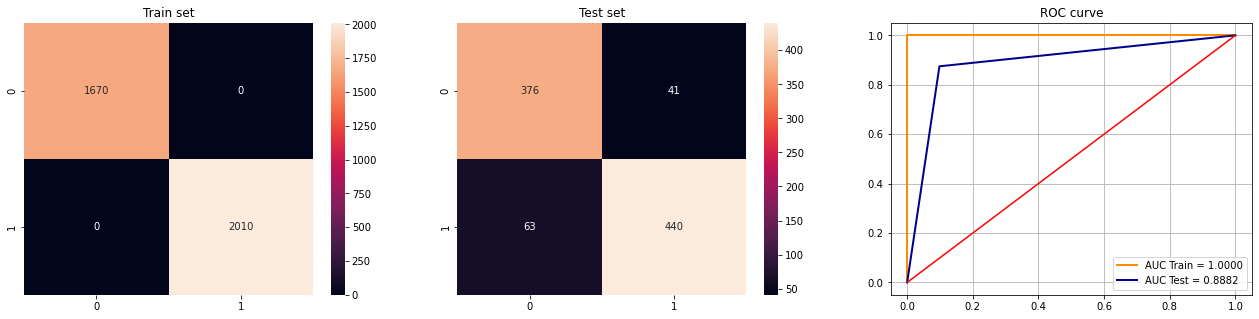
\includegraphics[width=\linewidth]{chapters/deteccion/images/dt.png}
        \caption{Métricas para el modelo de árbol de decisión}
        \label{fig.dt}
  \end{figure}
  
  En la Tabla \ref{tabla.dt} se detallan las métricas derivadas de la matriz de confusión. 

\begin{table}[H]
\centering
\begin{tabular}{|c|c|c|c|c|c|}
\hline
      & Accuracy & Precision & Recall & AUC    & $F_1$ score \\ \hline
Train & 1.0   & 1.0    & 1.0 & 1.0 & 1.0      \\ \hline
Test  & 0.887      & 0.9148    & 0.8748 & 0.8882  & 0.8943      \\ \hline
\end{tabular}
\caption{Métricas para el modelo de árbol de decisión}
\label{tabla.dt}
\end{table}

Comparando las métricas obtenidas para los conjuntos de entrenamiento y prueba, se evidencia claramente que el modelo sufre de sobreajuste. Aunque se podría haber intentado mitigar este sobreajuste mediante la optimización de hiperparámetros, se descartó esta opción debido a la disponibilidad de un modelo superior (random forest) y al considerable aumento en el tiempo de ajuste de dicho modelo.

\subsection{KNN}

Luego del entrenamiento se obtuvieron la matriz de confusión y curva roc tanto para train como para test, las cuales son mostradas en la Fig. \ref{fig.knn}. 

\begin{figure}[H]
\centering
        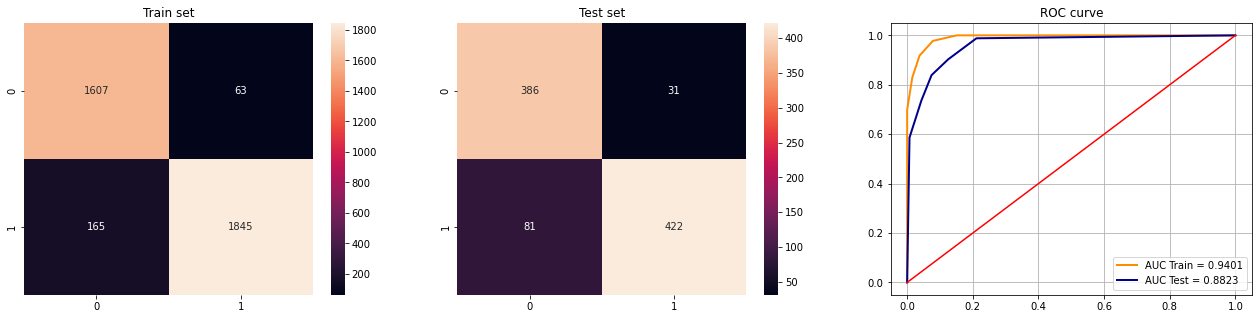
\includegraphics[width=\linewidth]{chapters/deteccion/images/knn.png}
        \caption{Métricas para el modelo KNN}
        \label{fig.knn}
  \end{figure}
  
  En la Tabla \ref{tabla.knn} se detallan las métricas derivadas de la matriz de confusión. 

\begin{table}[H]
\centering
\begin{tabular}{|c|c|c|c|c|c|}
\hline
      & Accuracy & Precision & Recall & AUC    & $F_1$ score \\ \hline
Train & 1.0   & 1.0    & 1.0 & 1.0 & 1.0      \\ \hline
Test  & 0.887      & 0.9148    & 0.8748 & 0.8882  & 0.8943      \\ \hline
\end{tabular}
\caption{Métricas para el modelo KNN}
\label{tabla.knn}
\end{table}


\subsection{Red neuronal convolucional}

Finalmente se aplicó un modelo de $\textit{deep learning}$, una red neuronal convolucional. Básicamente consta de cuatro bloques $\textit{convolucional}$, $\textit{batch normalization}$, $\textit{max pooling}$, una capa de $\textit{flatten}$ y luego tres bloques de capa $\textit{densa y dropout}$ como regularización. El optimizador utilizado fue $\textit{adam}$, la función de pérdida $\textit{binary crossentropy}$ tomando como métrica $\textit{accuracy}$ dado que el dataset estaba razonablemente balanceado. Se entrenó la red con un $\textit{batch size}$ de 10, $\textit{validation split}$ de 0.2 y con 100 $\textit{epochs}$.

Antes de calcular las métricas correspondientes de clasificación para este modelo, se procedió a investigar si hubo un overfitting durante el entrenamiento. Para esto se graficó la función de pérdida y el accuracy tanto de train como de test para cada epoch. La gráfica se muestra en la Fig. \ref{fig.loss}. 


\begin{figure}[H]
\centering
        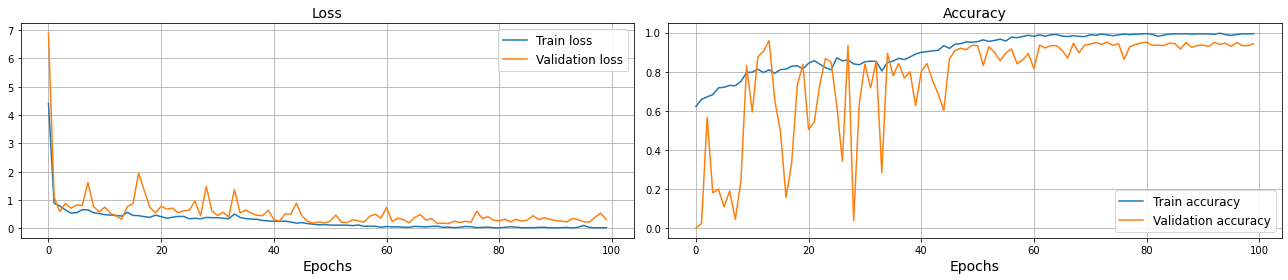
\includegraphics[width=\linewidth]{chapters/deteccion/images/loss.png}
        \caption{Función de pérdida y accuracy para el modelo de red convolucional.}
        \label{fig.loss}
  \end{figure}

Se observa que en principio no hay un overfitting. Al momento de calcular las predicciones, el modelo entrega una probabilidad de pertenecer a cada clase, por lo tanto se eligió un valor de umbral, el cual fue de 0.59, es decir, aquellas probabilidades mayores a 0.59 serían clasificadas como 1, es decir, con tumor y viceversa. El detalle de estos cálculos se encuentra en el código disponible en el Github. Una vez teniendo este valor umbral se calcularon las métricas, las cuales se muestran en la Tabla \ref{tabla.cnn} y en la Fig. \ref{fig.cnn_me}.


\begin{figure}[H]
\centering
        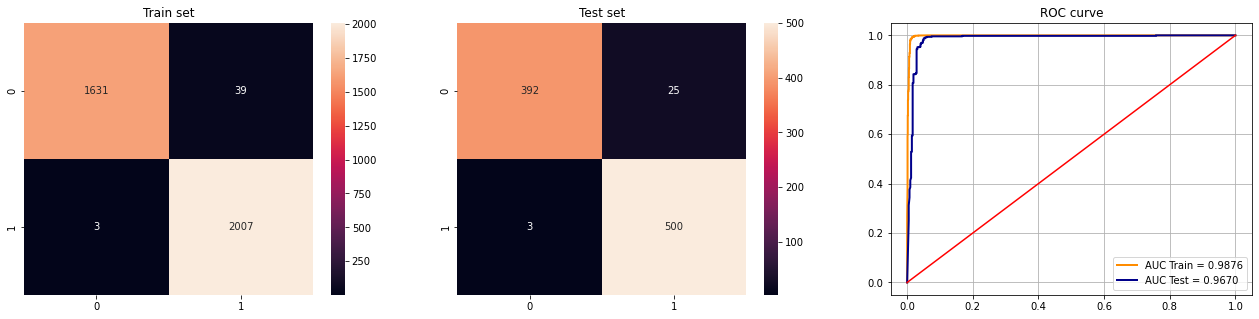
\includegraphics[width=\linewidth]{chapters/deteccion/images/cnn_met.png}
        \caption{Métricas para el modelo de red convolucional}
        \label{fig.cnn_me}
  \end{figure}

\begin{table}[H]
\centering
\begin{tabular}{|c|c|c|c|c|c|}
\hline
      & Accuracy & Precision & Recall & AUC    & $F_1$ score \\ \hline
Train & 0.9886   & 0.9809    & 0.9985 & 0.9876 & 0.9896      \\ \hline
Test  & 0.9696      & 0.9524    & 0.994 & 0.967  & 0.9728      \\ \hline
\end{tabular}
\caption{Métricas para el modelo de red convolucional}
\label{tabla.cnn}
\end{table}

\section{Resumen de modelos}

En términos de métricas, el mejor modelo pareciera ser el Random Forest, sin embargo, considero que el de red neuronal convolucional es mejor porque exhibe un mejor recall. 

En el contexto del problema, es importante no solo clasificar correctamente a los verdaderos positivos (pacientes efectivamente con tumores), sino también reducir los falsos negativos (pacientes con tumor pero clasificados como sanos).

Por este motivo, se optó por el modelo de redes neuronales convolucionales.











% Introducción

\chapter{Segmentación de tumores}

\section{Descripción del dataset}

\href{https://www.kaggle.com/datasets/pkdarabi/brain-tumor-image-dataset-semantic-segmentation} {Link} del dataset. 

Este dataset contiene 2146 imágenes con sus respectivas máscaras y está subdivivido en conjuntos de entrenamiento (1502 archivos), validación (429 archivos) y test (215).

 En la Fig. \ref{fig.mask} se observa la superposición de una imagen del dataset con su respectiva máscara, indicando la ubicación del tumor.
 
 
\begin{figure}[H]
\centering
        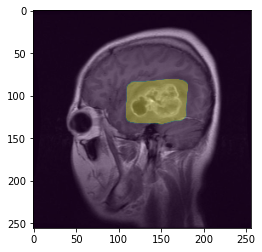
\includegraphics[width=0.3\linewidth]{chapters/segmentacion/images/mask.png}
        \caption{Imagen junto con la máscara indicando el tumor.}
        \label{fig.mask}
  \end{figure}


\section{Preprocesamiento de las imágenes}

Las imágenes disponibles tenían todas el mismo tamaño $(640\times640)$. Con el objetivo de normalizar las imágenes, se optó por redimensionarlas a una resolución de ($256 \times 256$) píxeles. 

Se aplicó una conversión a escala de grises, dado que esta representación es ampliamente utilizada en el ámbito del diagnóstico médico, garantizando así una compatibilidad estándar para el análisis y la interpretación de las imágenes.

Un último preprocesamiento que se aplicó es normalizar el rango de valores de los píxeles de la imagen, originalmente cada píxel $p_{ij}\in [0,255]$ y luego de la transformación $p_{ij}\in [0,1]$.

Las máscaras eran imágenes binarias del mismo tamaño que la imagen sobre la que segmenta. 


\section{Modelo: UNET}

Como modelo de segmentación se utilizó la red ampliamente utilizada UNET, cuya arquitectura se muestra en la Fig. \ref{fig.unet}. 

\begin{figure}[H]
\centering
        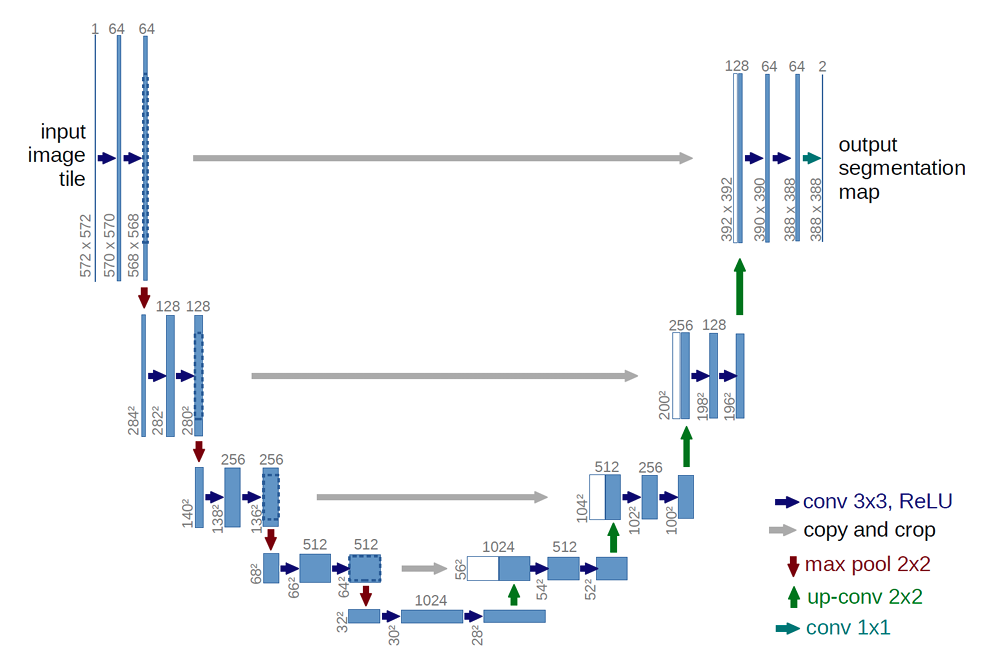
\includegraphics[width=0.7\linewidth]{chapters/segmentacion/images/unet.png}
        \caption{UNET}
        \label{fig.unet}
  \end{figure}

Esta arquitectura consta de un bloque de cuatro encoders, un bloque convolucional y un bloque de cuatro decoders. 

El optimizador utilizado fue $\textit{adam}$, la función de pérdida $\textit{dice loss}$ tomando como métrica $\textit{dice coefficient}$. Se entrenó la red con un $\textit{batch size}$ de 10, $\textit{validation split}$ de 0.2 y con 100 $\textit{epochs}$. Se implementó un callback de EarlyStopping. 

Dado que el target de este modelo es una máscara, una imagen, tenía más sentido tomar como función de pérdida el coeficiente de Dice, el cual se define como:

\begin{equation}
DSC(X,Y) = \frac{2|X\cap Y|}{|X|+|Y|}
\end{equation}.

Este coeficiente es igual a 1 si y solo si $X=Y$, y 0 si $X$ e $Y$ son no conexos. Esto codifica matemáticamente la superposición de la máscara obtenida con la máscara target. 

Antes de calcular las métricas correspondientes de clasificación para este modelo, se procedió a investigar si hubo un overfitting durante el entrenamiento. Para esto se graficó la función de pérdida y el accuracy tanto de train como de test para cada epoch. La gráfica se muestra en la Fig. \ref{fig.loss}. 


\begin{figure}[H]
\centering
        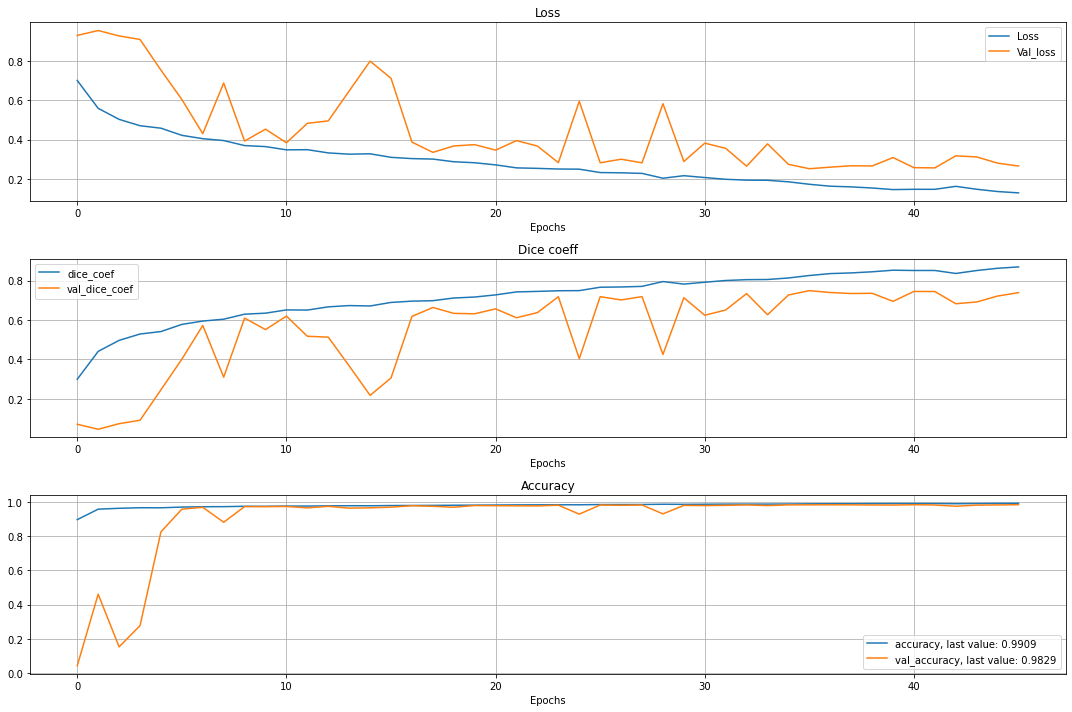
\includegraphics[width=0.8\linewidth]{chapters/segmentacion/images/metricas.png}
        \caption{Función de pérdidas y accuracy para la red UNET.}
        \label{fig.loss}
  \end{figure}

Observando las gráficas anteriores se observa que el modelo no overfitea. 

A continuación se procedió a calcular las métricas correspondientes. En este caso se calculó el coeficiente de Dice para cada conjunto de datos, los cuales se muestran en la Fig. \ref{fig.dice}.


\begin{figure}[H]
\centering
        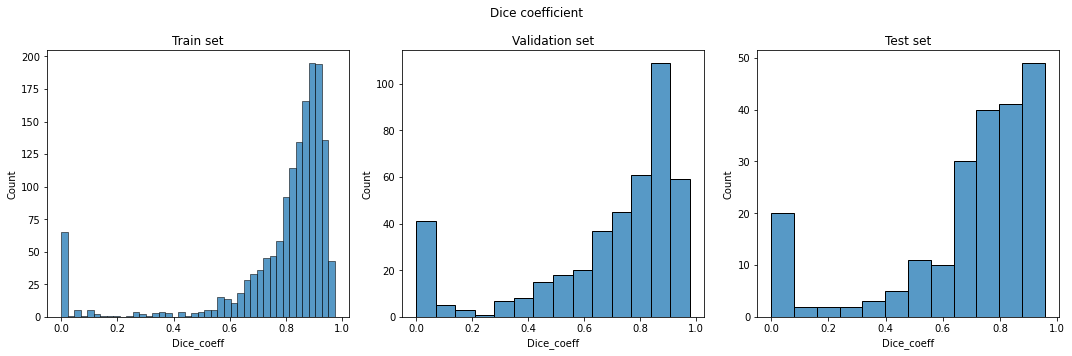
\includegraphics[width=0.9\linewidth]{chapters/segmentacion/images/dice.png}
        \caption{Coeficiente de Dice para cada conjunto de imágenes.}
        \label{fig.dice}
  \end{figure}

Se observa que en todos los casos, el valor máximo de la distribución está cercano a uno, indicando que el modelo funcionó razonablemente bien. Es notable observar que existen algunos coeficientes menores que uno. Esto se explica considerando que las máscaras usadas como target eran perfectamente rectangulares, mientras que las máscaras predichas por el modelo no lo son, sino que intentan adaptarse al tumor copiando su forma, como se observa en la Fig. \ref{fig.imagenes}. 

En el código subido a Github está el detalle de los cálculos realizados, así como un slider para poder ver las imágenes con sus correspondientes máscaras.

\begin{figure}[H]
    \centering
    \begin{subfigure}{0.45\textwidth}
        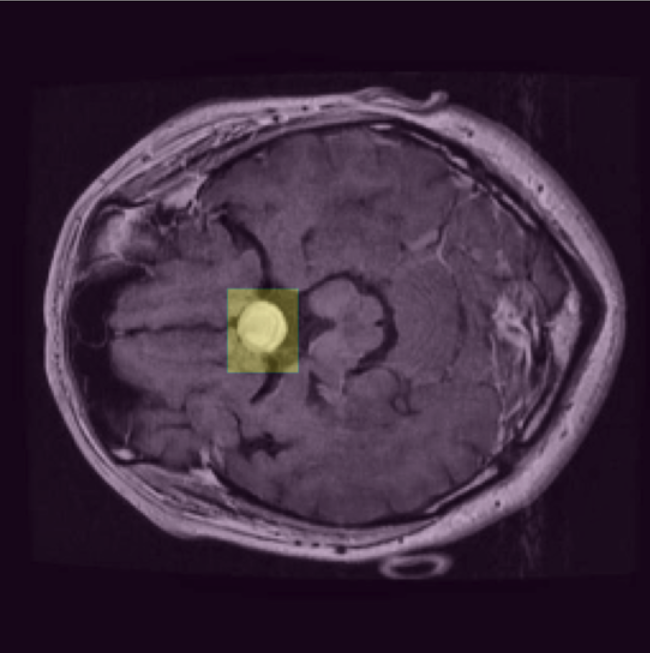
\includegraphics[width=\linewidth]{chapters/segmentacion/images/1.png}
        \caption*{}
    \end{subfigure}
    \hfill
    \begin{subfigure}{0.45\textwidth}
        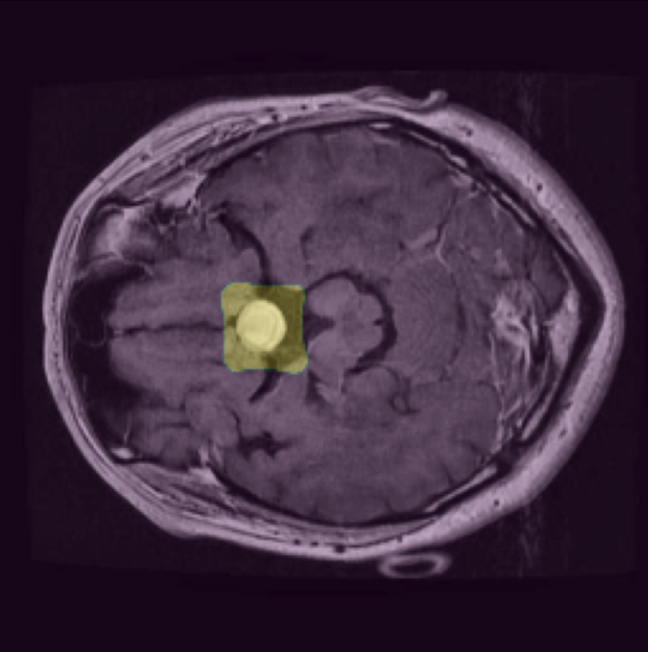
\includegraphics[width=\linewidth]{chapters/segmentacion/images/2.png}
        \caption*{}
    \end{subfigure}
    \medskip
    
    \begin{subfigure}{0.45\textwidth}
        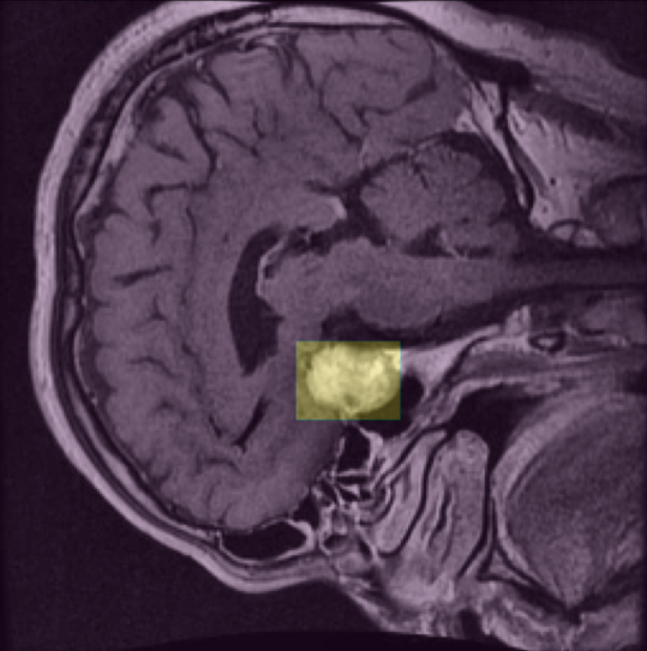
\includegraphics[width=\linewidth]{chapters/segmentacion/images/3.png}
       \caption*{}
    \end{subfigure}
    \hfill
    \begin{subfigure}{0.45\textwidth}
        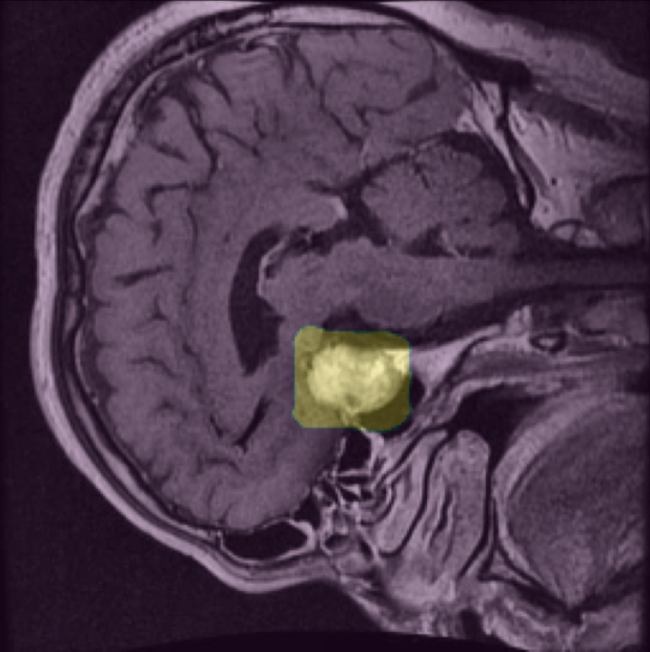
\includegraphics[width=\linewidth]{chapters/segmentacion/images/4.png}
        \caption*{}
    \end{subfigure}
    \medskip
    
    \begin{subfigure}{0.45\textwidth}
        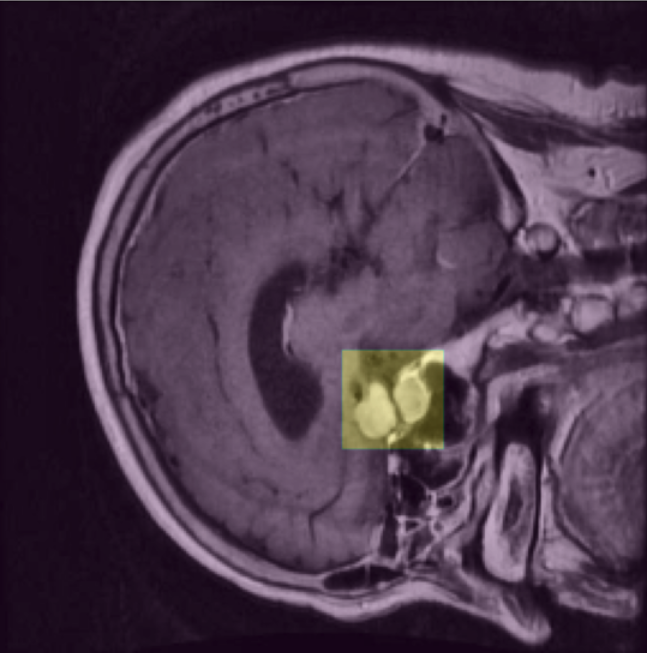
\includegraphics[width=\linewidth]{chapters/segmentacion/images/5.png}
        \caption*{Máscaras target}
    \end{subfigure}
    \hfill
    \begin{subfigure}{0.45\textwidth}
        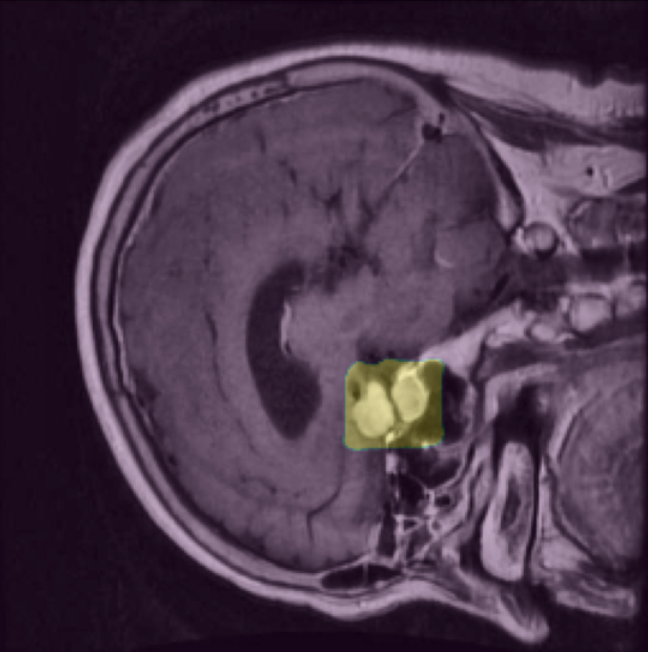
\includegraphics[width=\linewidth]{chapters/segmentacion/images/6.png}
       \caption*{Máscaras predichas}
    \end{subfigure}
    \caption{Comparación de máscaras dadas y predichas por el modelo}
    \label{fig.imagenes}
\end{figure}
















% Introducción

\chapter{Puesta en producción y conclusiones}

Habiendo desarrollado y validado los modelos de detección y segmentación de tumores, se procedió a poner en producción ambos modelos. Esto se llevó a cabo en etapas:

\begin{itemize}

\item construcción de API para detección,
\item construcción de API para segmentación,
\item construcción de front end sencillo,
\item dockerización.
\end{itemize}

El flujo de información sería el siguiente:

\begin{enumerate}
    \item se carga una imagen,
    \item la imagen se guarda y se da la opción de cargar otra o procesarla con el primer modelo para detectar un tumor,
    \item si el tumor es detectado, se informa y se da la opción de aplicar el modelo de segmentación, mostrando la imagen con la máscara predicha,
    \item si el tumor no es detectado y se solicita su segmentación, se informa que no hay tumor a segmentar.
\end{enumerate}

A continuación se muestran imágenes del front end desarrollado y el procesamiento en la Fig. \ref{fig.web}.

El diseño del front end y back end responden al Modelo Vista Controlador usando FastAPI. Los detalles están en el Github. 

\begin{figure}[H]
    \centering
    \begin{subfigure}[b]{0.45\textwidth}
        \centering
        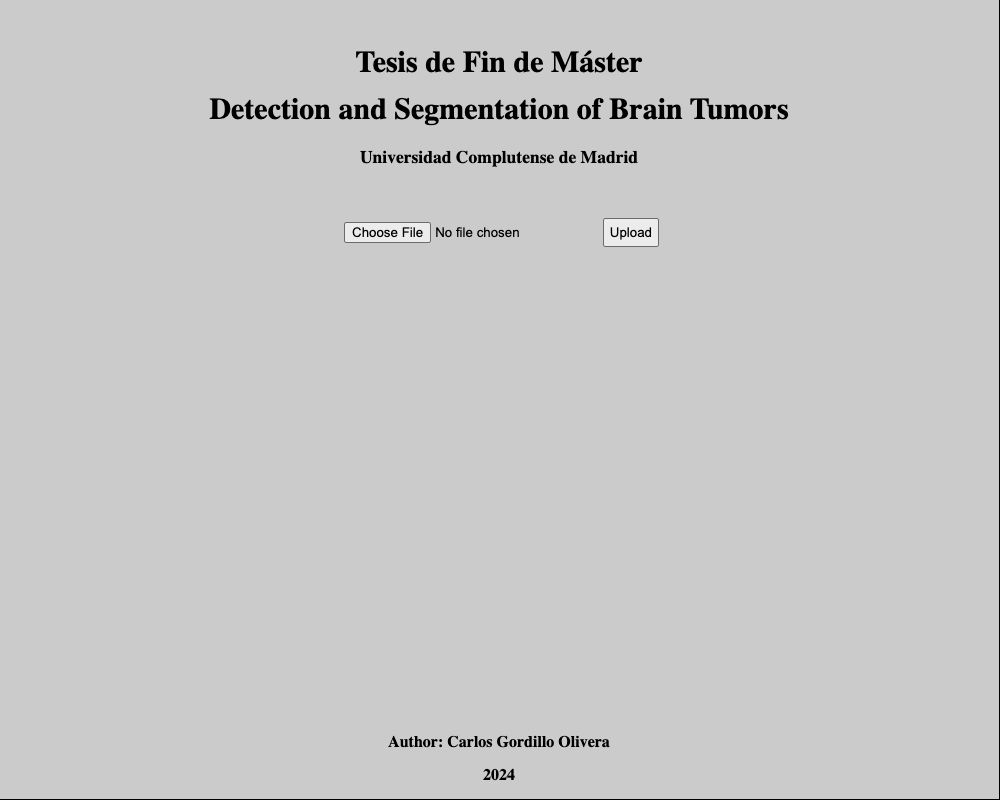
\includegraphics[width=\textwidth]{chapters/api/images/home.png}
        \caption{Vista inicial}
        \label{fig:imagen1}
    \end{subfigure}
    \hfill
    \begin{subfigure}[b]{0.45\textwidth}
        \centering
        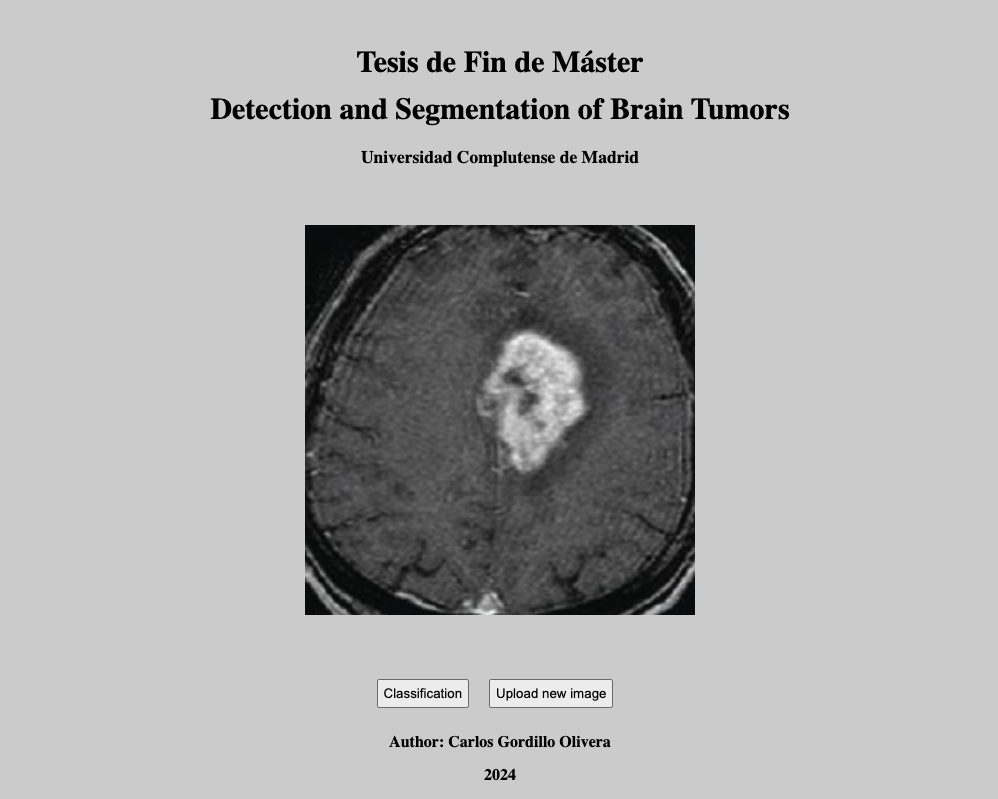
\includegraphics[width=\textwidth]{chapters/api/images/image.png}
        \caption{Imagen cargada}
        \label{fig:imagen2}
    \end{subfigure}
    
    \vspace{0.5cm} % Espacio vertical adicional entre las filas
    
    \begin{subfigure}[b]{0.45\textwidth}
        \centering
        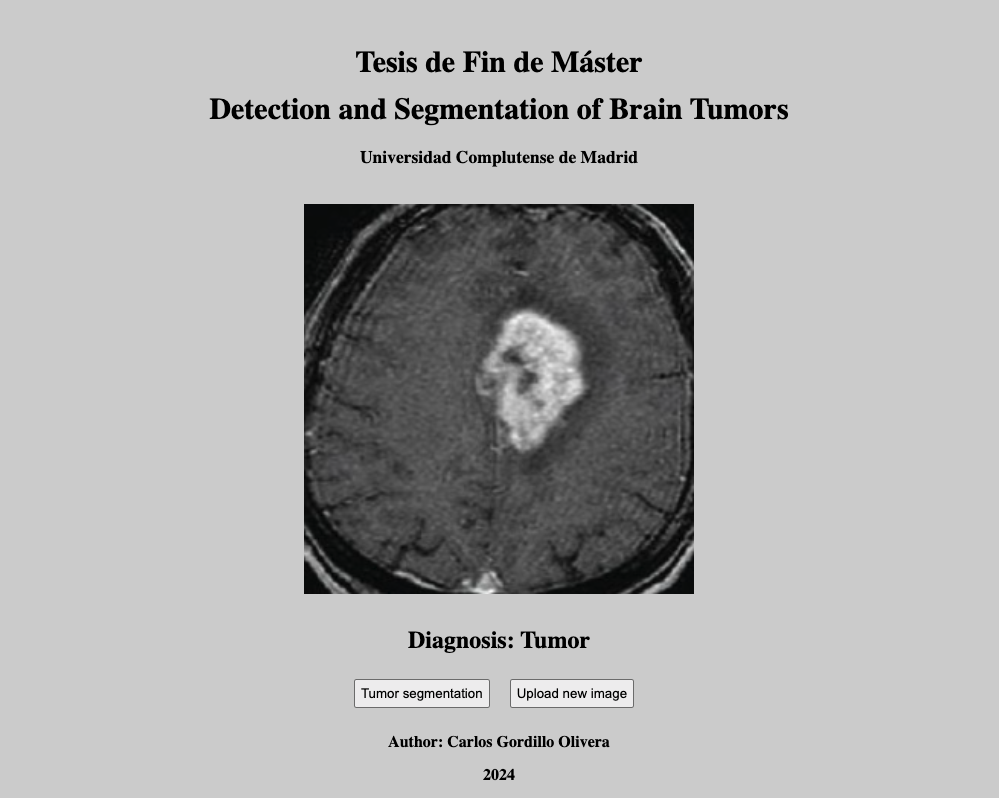
\includegraphics[width=\textwidth]{chapters/api/images/deteccion.png}
        \caption{Resultado de la detección}
        \label{fig:imagen3}
    \end{subfigure}
    \hfill
    \begin{subfigure}[b]{0.45\textwidth}
        \centering
        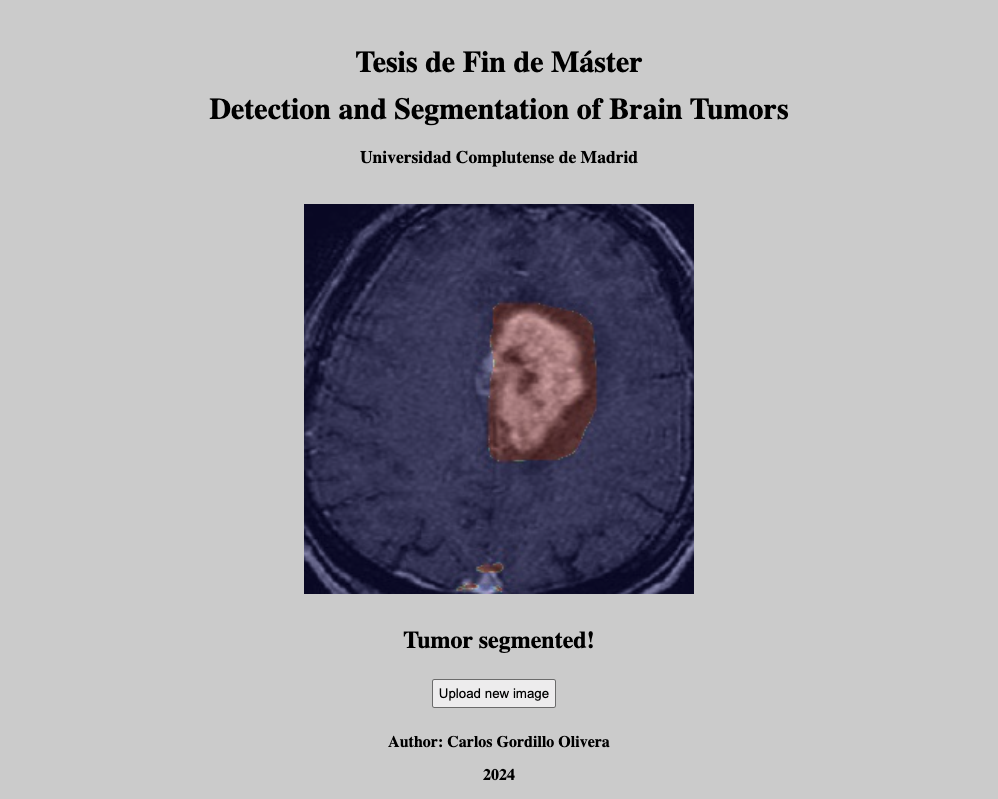
\includegraphics[width=\textwidth]{chapters/api/images/segmentacion.png}
        \caption{Resultado de la segmentación}
        \label{fig:imagen4}
    \end{subfigure}
    \caption{Flujo de información}
    \label{fig.web}
\end{figure}


Como conclusiones finales, se logró desarrollar un modelo de detección de tumores cerebrales. Dicho modelo fue evaluado y se descartó overfitting y presentó excelentes métricas de desempeño.

Se desarrolló también un modelo de segmentación de tumores, es decir, no únicamente detectar la presencia de tumores sino determinar la ubicación de los mismos. Se lo evaluó descartando overfitting y presentó buenas métricas.

Finalmente se desarrolló una API junto con un front end con el objetivo de poner en producción ambos modelos sumado a la visualización por parte del usuario. 

Como trabajo a futuro podría considerarse agregar un label más al target que identifique el tipo de imagen. Por ejemplo, en algunos casos el modelo segmentó como tumor a los ventrículos laterales en imágenes potenciadas en $T_2$, al ser el líquido brillante en estas imágenes, el algoritmo posiblemente los confundió con tumores en imagenes $T_1$ con contraste, donde también el tumor se ve brillante. 

Podría considerarse también aplicar data augmentation sobre la segmentación tumoral, pero no es tan sencillo porque no solo habría que realizar transformaciones sobre las imágenes usadas para entrenar, sino que la máscara target debería sufrir las mismas transformaciones.




% Bibliografía
\bibliography{bibliografia}

\end{document}
